\documentclass[t,aspectratio=169]{beamer}

\usepackage{soul}
\usepackage{tikz}
\usepackage{multicol}
\usepackage[utf8]{inputenc}

% ----------------------------------------------------------------------------------------------------------------------------------------

\title{\includegraphics[width=45pt]{oepecsetlogo.png}\\(KTXFI1EBNF) Physics I. Lecture}

\author{Dr.~Gábor FACSKÓ, PhD\\\tiny Assistant Professor / Senior Research Fellow\\\textit{facsko.gabor@uni-obuda.hu}}

\institute{\Tiny Óbuda University, Faculty of Electrical Engineering, 1084 Budapest, Tavaszmező u. 17.\\Wigner Research Centre for Physics, Department of Space Physics and Space Technology, 1121 Budapest, Konkoly-Thege Miklós út 29–33.\\ \url{https://wigner.hu/~facsko.gabor}}

\date{February 16,~2026}

\logo{\includegraphics[height=0.9 true cm]{kekcsik.png}}

% ----------------------------------------------------------------------------------------------------------------------------------------

\begin{document}

\frame{\titlepage}

% ----------------------------------------------------------------------------------------------------------------------------------------


\begin{frame}[fragile,squeeze,allowframebreaks]
\frametitle{Introduction}
\begin{itemize}
\setlength{\parskip}{0pt}
\setlength{\itemsep}{0pt}
\item Dr. Gábor István FACSKÓ (\texttt{facsko.gabor@uni-obuda.hu}) – I answer e-mails.
\item MSc in Physics and Astronomy, BSc in Computer Science – Eötvös Loránd University (ELTE)
\item Assistant Professor, Óbuda University, Faculty of Electrical Engineering, Budapest
\item Senior Research Fellow, Wigner Research Centre for Physics, Department of Space Physics, Budapest, \url{http://wigner.hu/~facsko.gabor}
\item Research interests: Space Plasma Physics, Computational Magnetohydrodynamics (MHD), Spacecraft Data Analysis
\item Career:
\begin{itemize}
\item 2008: PhD in Physics, Eötvös Loránd University, Budapest – Data Analysis
\item 2008–2010: \textit{LPC2E/CNRS, Orléans, France} – Instrumentation
\item 2010–2013: \textit{Finnish Meteorological Institute, Helsinki, Finland} – MHD Simulations
\item 2014–2018: \textit{Institute of Earth Physics and Space Science, Sopron, Hungary} – MHD Simulations; teaching MSc students at ELTE (Budapest) and University of Sopron
\pagebreak
\item 2018–2020: \textit{European Space Agency (ESA), Darmstadt, Germany} – Management, ISSI International Team member
\item \textbf{2020–present: Wigner Research Centre for Physics, Department of Space Physics, Budapest} – Computational MHD, Data Analysis, teaching Space Plasma Physics for MSc students in Physics, Astronomy, and Geophysics
\item 2022–2024: \textit{Milton Friedman University, Budapest} – Teaching Linux/UNIX, C\#, Python, SQL, and \LaTeX\ for BSc IT students
\item 2024–2025: \textit{University of Pecs, Faculty of Sciences, Institute of Mathematics and Informatics, Pecs} – Teaching Linear Algebra and Python for BSc students in IT, Mathematics, Physics, and Chemistry; founder of Pannon SpaceLab
\item 2024–2025: \textit{NASA Goddard Space Flight Center, Greenbelt, MD, USA} – External Contractor (Visiting Scientist in 2016, 2017, 2023)
\item \textbf{2025–present: Obuda University, Faculty of Electrical Engineering, Budapest}~–~Teaching (KTXFI1EBNF)~Physics~I., and (KTXFI2EBNF)~Physics~II. for BSc Electrical Engineering students in English
\end{itemize}
\pagebreak
\item Supervision of 1 MSc in Physics, 1 BSc in Physics, 3 BSc IT, and 1 TDK student + \textbf{ 1 PhD student in Oulu}
\item Questions:
\begin{itemize}
\item You know what lecture, practice, signature, test, and exam mean, don’t you?
\item Do you know what a Scientific Students’ Conference (TDK) is?
\item Did you know that you can start a PhD after a BSc in the UK, USA, or Australia?
\end{itemize}
\item Special services:
 \begin{itemize}
\setlength{\parskip}{0pt}
\setlength{\itemsep}{0pt}
\item BSc and TDK thesis topics
\item Career advice (over 1400 contacts on Facebook and LinkedIn), \textbf{Master Plan}
\item Soft skills training (CVs, motivation letters, presentations, networking)
\end{itemize}
\item Lectures and practices recorded with OBS Studio and a mobile phone, uploaded to Moodle/Teams
\item All slides, homeworks, tests, and exams will be available on Moodle/Teams, \underline{\href{https://github.com/gfacsko}{GitHub}}, and my \underline{\href{https://www.youtube.com/@gaborfacsko4971}{YouTube.com}} channel
\end{itemize}
\end{frame}

% ----------------------------------------------------------------------------------------------------------------------------------------

\begin{frame}[fragile,squeeze,allowframebreaks]
\frametitle{Course Objectives}
The purpose of the subject is the establishment, organization, and integration of the foundations of physics into a unified framework, and the transfer of all these to university students. The aim is the acquisition of specific knowledge by students through the foundation. In general, this helps in better understanding technical problems by approaching the phenomena from another (physical, and not technical) perspective. The subject lays the foundation for the subsequent modern physics (Physics II) subject. The main educational objective of the subject is the development of students’ technical problem-solving thinking. The achievement of the mentioned goals is intended to be reached through university lectures and calculation exercises.  
\pagebreak
\normalsize
\begin{enumerate}
\setlength{\parskip}{0pt}
\setlength{\itemsep}{0pt}
\item \textbf{Mechanics I.:} \textit{Newton’s laws, equation of motion (review). Momentum. General concept of mechanical work, work theorem. Forms of mechanical energy.}
\item \textbf{Mechanics II.:} \textit{Weight force, gravitational force, gravitational field. Work of the gravitational force. Conservative force field. Dissipative force field. Mechanical power.}
\item \textbf{Mechanics of Rigid Bodies I.} Concept of a rigid body. Forces acting on a rigid body. Motion of a rigid body. Concept of the centre of mass. Location of the centre of mass. Torque. Angular momentum. Energy of a rotating rigid body, angular momentum of a rotating rigid body, Steiner’s theorem. 
\item \textbf{Mechanics of Rigid Bodies II.} Principal theorems of rigid body motion; conservation laws. Collisions.
\item \textbf{Oscillations I.} Dynamic condition of harmonic oscillatory motion. Differential equation of harmonic undamped oscillatory motion.
\pagebreak
\item \textbf{Oscillations II.} Superposition of oscillations. Decomposition of oscillations into components. Damped oscillations. Forced oscillations, resonance. Coupled oscillations.
\item \textbf{Wave phenomena:} Reflection of waves, refraction of waves, diffraction of waves. Huygens–Fresnel principle. Interference of waves. Polarization of waves.
\item \textbf{Elements of acoustics:} Basics of acoustics. Fundamental concepts. Doppler effect. Sound intensity, loudness according to Weber–Fechner’s law.
\item \textbf{Thermodynamics I:} Temperature scales, thermal expansion, thermometers. State variables, ideal gas, state changes, ideal gas equation of state, Boyle’s law, Gay-Lussac’s laws, universal (combined) gas law, heat, specific heat, molar heat, heat capacity.
\item \textbf{Thermodynamics II:} Expansion work, internal energy, the first law of thermodynamics, forms of the first law in different state changes.
\pagebreak
\vskip -10 pt
\item \textbf{Thermodynamics III:} Cyclic processes, Carnot cycle, Carnot’s theorem, reduced heat, entropy, the second law of thermodynamics.
\item \textbf{Thermodynamics IV:} Kinetic theory of gases, molecular thermodynamics. Distributions, distribution functions. Elementary statistics.
\item \textbf{Electrostatics I.:} Electric charge: Fundamental electrical phenomena, electric charge and matter, Coulomb’s law (force between two point charges, unit of electric charge, permittivity of vacuum).
\item \textbf{Electrostatics II.:} The electric field: The electrostatic field (electric field strength, electric field lines). Determination of electric field strength. Gauss’s law (flux of the electric field). Electric field of a point charge.
\pagebreak
\item \textbf{Electrostatics III.:} Electrostatic potential: Work of the electric field (work done in an electric field). Electric potential (electrostatic potential). Electric potential difference, voltage. Electric potential of charge systems at small and large distances. Electrostatic energy.
\item \textbf{Elements of physical or wave optics.} Branches of optics. Light interference, light diffraction, diffraction through a slit, optical grating, light polarization. Light as an electromagnetic wave: Poynting vector. Optical instruments.
\end{enumerate}
\end{frame}

% ----------------------------------------------------------------------------------------------------------------------------------------

\begin{frame}[fragile,squeeze,allowframebreaks]
\frametitle{Requirements}
Students who fully comply with all of the points listed below during the semester may get a signature:
\begin{itemize}
\setlength{\parskip}{0pt}
\setlength{\itemsep}{0pt}
\item \st{The number of absences from lectures and exercises during the semester did not exceed the limit specified in the TVSZ (maximum 30\% of the total number of hours held).}
\item Correctly completed \st{4} 3 of the \st{6} 5 assigned homework assignments, submitted on time and in the required  format.
\item Achieved a score of at least 40\% on the midterm exam.
\item Extra credit: In addition to the homework assignments submitted during the semester, two more assignments can be submitted as extra credit. If the result of the assignment submitted in this way is correct, the student will receive +10 semester points per assignment. In this way, a maximum of +20 semester points can be earned with extra assignments, which will be included in the final semester score. \st{The extra credit assignment can be submitted either during the two weeks of the given homework assignment or, at the latest, during the week designated for making up homework assignments (see below for make-up assignments in the 13th week of instruction).}
 \pagebreak
\item Midterm exam: A poorly written or incorrect midterm exam with a score above 40\% cannot be corrected, i.e., it cannot be retaken for the purpose of correction. There is no retake exam. The score received for the extra credit assignment cannot be added to the score obtained on the midterm exam, i.e., the 40\% midterm exam score must be achieved solely from the midterm exam assignments.
\item Grades: Insufficient/Fail (1): 0-50\,\%, Sufficient/Pass (2): 51-60\,\%, Average (3): 61-75\,\%, Good (4): 76-90\,\%, Excellent (5): 91-\,\%.
\end{itemize}
\textbf{Recommended}\\
\textit{Richard P. Feynman: The Feynman Lectures on Physics, Vol. I: The New Millennium Edition: Mainly Mechanics, Radiation, and Heat, New York, 2010, ISBN-10 0465024939, IBN-13 978-0465024933}
\end{frame}

% ----------------------------------------------------------------------------------------------------------------------------------------

\begin{frame}%[fragile,squeeze,allowframebreaks]
\frametitle{An offer you can’t refuse}
\begin{itemize}
\setlength{\parskip}{0pt}
\setlength{\itemsep}{0pt}
\item I was offered a job on February 10, 2026 at the International Space University (\underline{\href{https://www.isunet.edu/}{ISU}}), Illkirch-Graffenstaden, France
\item It is a CDD (Contrat à Durée Déterminée) job for six months. My duties are
\begin{itemize}
\item Teaching a course at ISU from \textbf{March 9 to April 30, 2026}
\item Organize the 38th Space Studies Program (\underline{\href{https://www.isunet.edu/ssp/}{SSP}}) from \textbf{June 22 to August 14, 2026}
\end{itemize}
\item I suggest accelerating this course. I will teach 1+3+3 lectures and practice sessions on February 16, 23, and March 2, 2026. Then I will return and finish the course on May 4 and 11, 2026.
\item The midterm exam will be held on May 18, 2026 during the course slot.
\item \textbf{What do you think?}
\end{itemize}
Some background information: Only two English-speaking students of mine failed out of 33 last semester. 60 Hungarian students failed out of 80 in Prof.~Ervin~RÁCZ's course at the same time.
\end{frame}

% ----------------------------------------------------------------------------------------------------------------------------------------


\begin{frame}[fragile,squeeze,allowframebreaks]
\frametitle{Classical Mechanics}
\begin{itemize}
\item Introduction
\item Mechanics can be divided into three main chapters:
\begin{itemize}
\item Kinematics: answering the question how the body moves
\item Dynamics: answering the question why the body moves
\item Statics: studying physical systems in equilibrium with its environment
\end{itemize}
\item In this chapter we will investigate the main concepts present in Classical Dynamics.

\pagebreak 
\item The simplest mechanical system is, when a body moves under influence of no force, the so called \emph{free particle}.
\begin{center}
\begin{figure}
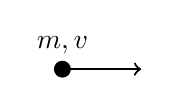
\begin{tikzpicture}[domain=0:4]
\filldraw[color=black] (0,0) circle (0.1);
\draw[color=black, thick,->] (0,0) -- (1,0);
\path(0,0.3) [black] node {$m,v$};
\end{tikzpicture}
\caption{Free particle with mass $m$ traveling through space at finite constant velocity $v$.}
\end{figure}
\end{center}
Two quantities are corresponded to the particle
\begin{enumerate}
\item kinetic energy: $E=\frac{1}{2}mv^{2}$
\item momentum
\end{enumerate}
\item We define the notion of \emph{dispersion relation}, a connection between energy, mass and momentum. In case of free particle, this relation is as follows


\pagebreak

\item Dispersion relation
\begin{columns}
\begin{column}{0.5\textwidth}
\begin{center}    
\begin{eqnarray*}
p&=&mv \\
p^{2}&=&m^{2}v^{2} \\
\frac{p^{2}}{2m}&=&\frac{1}{2}mv^{2} \\
E&=&\frac{p^{2}}{2m}
\end{eqnarray*}
\end{center}
\end{column}
\begin{column}{0.5\textwidth}
\begin{center}
\begin{figure}
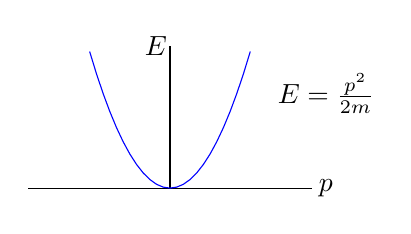
\begin{tikzpicture}[scale=0.6]
\draw (-3,0) -- (3,0);
\draw (0,0) -- (0,3);
\path (-0.3,3) [black] node {$E$};
\path (3.3,0) [black] node {$p$};
\draw[color=blue, domain=-1.7:1.7]    plot (\x,{(\x)^2});
\path (3.3,2) [black] node {$E=\frac{p^{2}}{2m}$};
\end{tikzpicture}
\caption{Dispersion relation for free particle.}
\end{figure}
\end{center}
\end{column}
\end{columns}

\pagebreak
\item Newton's laws of motion
\begin{enumerate}
\item A body is at rest or follows a straight path with a constant velocity, if there is no force acting on it.(\emph{Law of inertia})
\item Change in the body's momentum is a result of the force acting on it (\emph{Fundamental law of Dynamics})
$$F=\frac{dp}{dt}=\frac{d(m_{i}v)}{dt}=m_{i}\frac{dv}{dt}=m_{i}a.$$
\item If two bodies exert forces on each other, these forces have the same magnitude but opposite directions.(\emph{Law of action and reaction})
\end{enumerate}
\item $m_{i}$ denotes the \emph{inertial} mass of the body, indicating its resistance against force. Moreover we assumed a constant mass.

\pagebreak

\item Conservation of momentum: If there is no force acting on the body, then its momentum is constant
$$F=\frac{dp}{dt}, \text{if}\hspace{4.0 mm}F=0, \Longrightarrow p=\text{const.}$$

\item \emph{Work} ($W$) done by a force
\begin{eqnarray*}
\text{work}&=&\text{force}\cdot\text{displacement}, \\
W&=&F\cdot s,
\end{eqnarray*}
where $F$ is the force, and $s$ is the displacement.
\item Now let us imagine a particle at point $A$ with velocity $v_{A}$ and is influenced by a force $F$ translating it to point $B$, where its velocity $v_{B}$.

\pagebreak
\item Work-energy principle
\begin{center}
\begin{figure}
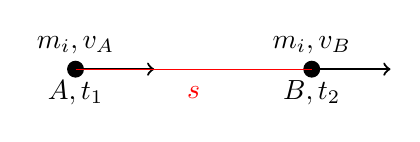
\begin{tikzpicture}
\filldraw[color=black] (0,0) circle (0.1);
\draw[color=black, thick,->] (0,0) -- (1,0);
\path(0,0.3) [black] node {$m_{i},v_{A}$};
\path(0,-0.3) [black] node {$A,t_{1}$};
\filldraw[color=black] (3,0) circle (0.1);
\path(3,0.3) [black] node {$m_{i},v_{B}$};
\path(3,-0.3) [black] node {$B,t_{2}$};
\draw[color=black, thick,->] (3,0) -- (4,0);
\draw[color=red, thin] (0,0) -- (3,0);
\path(1.5,-0.3) [red] node {$s$};
\end{tikzpicture}
\end{figure}
\end{center}
$ W_{AB}=\int\limits_{A}^{B}Fds=m_{i}\int\limits_{A}^{B}\frac{dv}{dt}\frac{ds}{\textcolor{blue}{dt}}\textcolor{blue}{dt}=m_{i}\int\limits_{t_{1}}^{t_{2}}\frac{dv}{dt}vdt=\int\limits_{t_{1}}^{t_{2}}\frac{d}{dt}\left(\frac{1}{2}m_{i}v^{2}\right)dt=\frac{1}{2}m_{i}v_{B}^{2}-\frac{1}{2}m_{i}v_{A}^{2}$
\item Observation: \emph{Work done on a body changes its kinetic energy}.

\pagebreak
\item Conservation of Mechanical Energy
\begin{eqnarray*}
\frac{d(m_{i}v)}{dt}&=&F \\
m_{i}\frac{dv}{dt}v&=&Fv \\
\frac{d}{dt}\left(\frac{1}{2}m_{i}v^{2}\right)&=&-\frac{d\phi}{dx}\frac{dx}{dt} \\
\frac{d}{dt}\left(\frac{1}{2}m_{i}v^{2}+\phi\right)&=&0 \\
\frac{1}{2}m_{i}v^{2}+\phi&=&\text{const.}=E
\end{eqnarray*}

\pagebreak
\item Observation: If the force $F$ can be written as a derivative of a function $\phi$ (potential energy). Then \emph{the sum of the kinetic and potential energy is constant during the motion}. This constant is called \emph{mechanical energy}.

\pagebreak
\item Gravity is one of the three interactions in Nature and like any other interaction, it has \emph{universal} characteristics.
\begin{columns}
  \begin{column}{0.4\textwidth}
\item Johannes Kepler
\begin{itemize}
    \item Student of Tycho Brahe
    \item Analysed data of Mars' orbit
    \item \emph{The orbit of a planet is an ellipse with the Sun at one of the two focuses.}
    \end{itemize}
  \end{column}
  \begin{column}{0.5\textwidth}
    \vfill
\begin{center}    
  \includegraphics[width=0.5\linewidth]{images-20260216/kepler.jpg}
\end{center}
\end{column}
\end{columns}

\pagebreak
\begin{columns}
\begin{column}{0.4\textwidth}
\item Sir Isaac Newton
\begin{itemize}
 \item 1687 \emph{Principia Mathematica}, describes \emph{universal} law of gravity via \emph{geometry}
 \item Orbits of physical objects around the Sun are \emph{conic sections}
 \item Unifies "celestial" and "earthly" physics, how? 
\end{itemize}
%
\end{column}
\begin{column}{0.5\textwidth}
  \vfill
  \begin{center} 
    \includegraphics[width=0.7\linewidth]{images-20260216/newton.jpg}
    \end{center} 
\end{column}
\end{columns}

\pagebreak
\item Same laws
\begin{columns}
\begin{column}{0.45\textwidth}
\centering
\includegraphics[width=0.8\linewidth]{images-20260216/water.jpg}\\
Water flow's orbit is parabola\\
\end{column}
\begin{column}{0.45\textwidth}
\centering
\includegraphics[width=0.5\linewidth]{images-20260216/solarsys.png}\\
Planetary orbits\\
\end{column}
\end{columns}

\pagebreak
\item Same laws (cont'd)
\begin{columns}
\begin{column}{0.4\textwidth}
\begin{itemize}
 \item Bodies moving in Earth's gravitational field follow parabolic curves
 \item Planets moving in Sun's gravitational field follow elliptic curves
 \item Worlds are unified via \emph{gravity}
\end{itemize}
\end{column}
\begin{column}{0.5\textwidth}
\vfill
\centering
\includegraphics[width=0.7\linewidth]{images-20260216/Conic.png}\\
Conic sections
\end{column}
\end{columns}

\pagebreak
\item Experiment
\begin{columns}
\begin{column}{0.4\textwidth}
\centering
\includegraphics[width=0.75\linewidth]{images-20260216/galilei.jpg}\\
Galileo Galilei
\end{column}
\begin{column}{0.45\textwidth}
\centering
\includegraphics[width=0.8\linewidth]{images-20260216/apollo15.jpg}\\
David Scott on Apollo 15 mission
\end{column}
\end{columns}

\pagebreak
\item Experiment (cont'd)
\begin{columns}
\begin{column}{0.5\textwidth}
\begin{itemize}
\item Bodies in free fall accelerate at \emph{the same rate}
\item \emph{independent from material quality}
\item {\color{red}{Gravity is a geometric interaction}}
\end{itemize}
\end{column}
\begin{column}{0.5\textwidth}
  \vfill
\centering
\includegraphics[width=0.7\linewidth]{images-20260216/whale.jpg}\\
A whale and a ball of petunia in free fall
\end{column}
\end{columns}

\pagebreak
\item Newton's law of universal gravitation law
\item Let us consider two bodies with masses $M_{1},M_{2}$ seperated by distance $r$. The gravitational force between them described by Newton's law of universal gravitation
\begin{center}
\begin{figure}
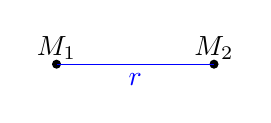
\begin{tikzpicture}[domain=0:4]
\filldraw[color=black] (-1,0) circle (0.05);
\filldraw[color=black] (1,0) circle (0.05);
\draw[color=blue] (-1,0) -- (1,0);
\path(0,-0.2) [blue] node {$r$};
\path(-1,0.2) [black] node {$M_{1}$};
\path(1,0.2) [black] node {$M_{2}$};
\end{tikzpicture}
\caption{Two bodies in gravitational interaction.}
\end{figure}
\end{center}
\vskip -10 pt
\begin{alertblock}{Newton's gravitational law}
  \vskip -10 pt
  $$F_{gr}=-G\frac{M_{1}M_{2}}{r^{2}},$$
where $G=6.67\cdot 10^{-11}\frac{m^{3}}{kgs^{2}}$ is Newton's gravitational constant.
\end{alertblock}

\pagebreak
\item Work-energy principle
\begin{columns}
\begin{column}{0.5\textwidth}  
\begin{center}
\begin{figure}
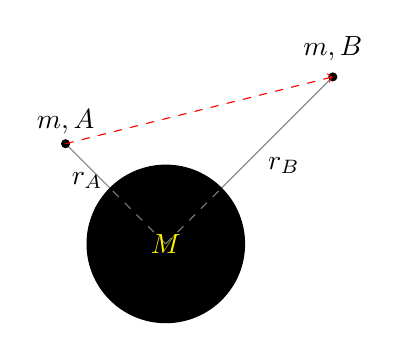
\begin{tikzpicture}[domain=0:4]
\draw[color=gray] (0,0) -- ({3*cos(45},{3*sin(45)});
\draw[color=gray] (0,0) -- ({1.8*cos(135},{1.8*sin(135)});
\filldraw[color=black] (0,0) circle (1);
\draw[color=gray, dashed] (0,0) -- ({1*cos(135},{1*sin(135)});
\draw[color=gray, dashed] (0,0) -- ({1*cos(45},{1*sin(45)});
\path(0,0) [yellow] node {$M$};
\filldraw[color=black] ({1.8*cos(135},{1.8*sin(135)}) circle (0.05);
\filldraw[color=black] ({3*cos(45},{3*sin(45)}) circle (0.05);
\draw[color=red,dashed,->] ({1.8*cos(135},{1.8*sin(135)}) --({3*cos(45},{3*sin(45)});
\path({1.8*cos(135},{2.2*sin(135)}) [black] node {$m,A$};
\path({3*cos(45},{3.5*sin(45)}) [black] node {$m,B$};
\path(-1,0.8) [black] node {$r_{A}$};
\path(1.5,1) [black] node {$r_{B}$};
\end{tikzpicture}
\caption{Work done by gravity.}
\end{figure}
\end{center}
\end{column}
\begin{column}{0.5\textwidth}
$W_{AB}=\int\limits_{A}^{B}-G\frac{mM}{r^{2}}dr=-GmM\int\limits_{A}^{B}\frac{dr}{r^{2}}=-GmM\left(\frac{1}{r_{A}}-\frac{1}{r_{B}}\right)$
$$\textcolor{blue}{W_{AB}=-\frac{GmM}{r_{A}}+\frac{GmM}{r_{B}}}$$
\end{column}
\end{columns}

\pagebreak
\item Work-energy principle (cont'd)
\begin{itemize}
\item if $r_{B}\rightarrow\infty$, we define the \emph{gravitational potential energy} of the body at point A: $E_{pot}=-\frac{GmM}{r_{A}}$ 
\item According to work-energy principle, the work done by gravity changes the body's kinetic energy
\end{itemize}
\item {\color{red}{Work-energy principle in presence of gravity}}
\begin{eqnarray*}
\frac{1}{2}mv_{A}^{2}-\frac{GmM}{r_{A}}&=&\frac{1}{2}mv_{B}^{2}-\frac{GmM}{r_{B}}, \\
\frac{1}{2}mv^{2}-\frac{GmM}{r}&=&\text{const.}=E.
\end{eqnarray*}
\item {\color{blue}{Mechanical energy is conserved in gravitational interaction. Gravity is a conservative force.}}

\pagebreak
\item \underline{Escape velocity:} As an application for work-energy principle, we consider the following scenario. A rocket tries to leave the gravitational field of a planet. What velocity is required for this? This quantity is called \emph{the 2nd celestial} or \emph{escape velocity}.
\begin{columns}
\begin{column}{0.6\textwidth}
\begin{center}
\begin{figure}
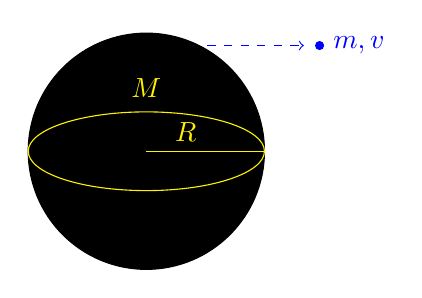
\begin{tikzpicture}
\filldraw[color=black] (0,0) circle (1.5);
\draw[yellow] (0,0) ellipse (1.5 and 0.5);
\draw[yellow] (0,0) -- (1.5,0);
\path(0.5,0.25) [yellow] node {$R$};
\path(0,0.8) [yellow] node {$M$};
\draw[color=blue,dashed,->] ({1.55*cos(60)},{1.55*sin(60)}) -- (2,{1.55*sin(60)});
\filldraw[color=blue] (2.2,{1.55*sin(60)}) circle (0.05);
\path(2.7,{1.55*sin(60)}) [blue] node {$m,v$};
\end{tikzpicture}
\caption{A rocket trying to escape from a planet's gravitational field.}
\end{figure}
\end{center}
\end{column}
\begin{column}{0.4\textwidth}
\begin{center}
The condition for this velocity is 
$$\frac{1}{2}mv^{2}-\frac{GmM}{R}=0$$
$$v=\sqrt{\frac{2GM}{R}}.$$
\end{center}
\end{column}
\end{columns}

\pagebreak

\item \underline{A dissipative force field} is a non-conservative, velocity-dependent field that removes mechanical energy from a system, converting it into heat or internal, microscopic energy.
\item Common examples include friction, air resistance, and viscous drag, which always oppose motion. These forces are essential in modeling systems that evolve toward equilibrium.
\item Key Characteristics of Dissipative Forces
\begin{itemize}
\item Energy Loss: They decrease the total mechanical energy of a system, converting it into non-recoverable forms like thermal energy.
\item Direction: They act opposite to the direction of motion (velocity vector).
\item Path Dependence: The work done by dissipative forces depends on the specific path taken, unlike conservative forces (e.g., gravity).
%\item Representation: Often modeled as  or through a Rayleigh dissipation function in Lagrangian mechanics.
\end{itemize}

\pagebreak
\item Common Examples and Contexts
\begin{itemize}
\item  Friction: Kinetic friction on a sliding object.
\item Fluid Resistance/Drag: Air resistance on a moving vehicle.
\item Viscosity: Internal friction within fluids.
\item Dissipative Particle Dynamics (DPD): A simulation technique for soft matter that uses conservative, random, and dissipative forces to model mesoscopic systems.
\end{itemize}
\item Unlike conservative forces, which act between macroscopic components, dissipative forces arise from the interaction between macroscopic motion and microscopic, random molecular motion (heat). In thermodynamics, they are central to "open" or non-equilibrium systems. 

\pagebreak
\underline{Mechanical power} is the rate at which work is done or mechanical energy is transferred, calculated as force multiplied by velocity ($P=\mathbf{F}\mathbf{v}$), or torque multiplied by angular velocity ($P=\mathbf{\tau}\mathbf{\omega}$), where $\mathbf{F}$ is the force, $\mathbf{v}$ is the velocity, and $\mathbf{\tau}=\mathbf{F}\times\mathbf{r}$, with $\mathbf{r}$ being the distance from the center to the point where the force is applied; finally, $\mathbf{\omega}$ is the angular velocity. It represents how fast a system can deliver energy and is commonly measured in watts (W).

\end{itemize}
\end{frame}

% ----------------------------------------------------------------------------------------------------------------------------------------

\begin{frame}
%\frametitle{Minden jó, ha a vége jó}

\vfill
\begin{center}
\textbf{\huge The End}

\bigskip
Thank you for your attention!
\end{center}
\vfill
\textbf{Acknowledgements} Thank you for the course materials for Szilárd~ZSÓKA and Zoltán~VARGA.
\end{frame}

\end{document}
